\documentclass{article}

% Formatting
\usepackage[utf8]{inputenc}
\usepackage[margin=1in]{geometry}
\usepackage[titletoc,title]{appendix}
\usepackage[spanish]{babel}
\usepackage{amsmath,amsfonts,amssymb,mathtools}
\usepackage{graphicx,float}
\usepackage[ruled,vlined]{algorithm2e}
\usepackage{algorithmic}
\usepackage{minted}
\usemintedstyle{borland}
\usepackage{biblatex}
\usepackage{subcaption}
\usepackage{multicol}
\usepackage{listings}
\usepackage{xcolor}
\addbibresource{ref.bib}


% Title content
\title{Práctica 2 Autómata Celular}
\author{Denisse Leyva}
\date{Febrero 24, 2021}

\begin{document}

\maketitle

% Introduction
\section{Introducción}
En esta segunda práctica trabajaremos con autómatas celulares en dos dimensiones, particularmente el famoso juego de la vida. El estado del autómata se representa con una matriz booleana (es decir, contiene ceros y unos). Cada celda es o viva (uno) o muerta (cero). En cada paso, la supervivencia de cada celda (verde) se determina a partir de los valores de sus ocho vecinos (amarillos):\\

\begin{multicols}{2}
\begin{figure}[H]
\centering
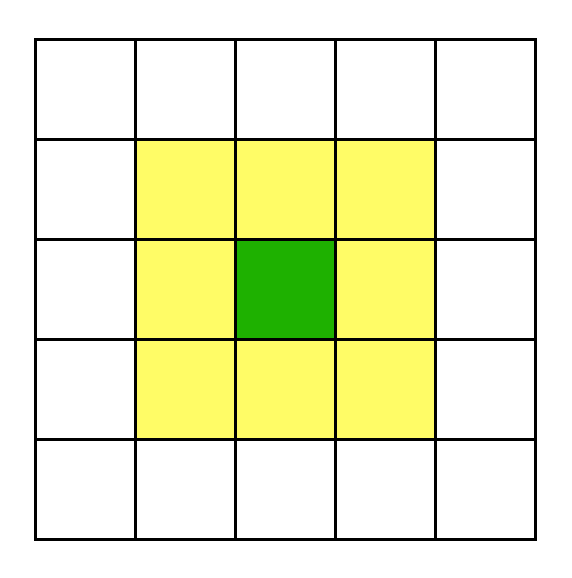
\includegraphics [width =0.3\textwidth]{p2v.png}
\caption{Matriz Booleana}
\end{figure}
\end{multicols}


En los extremos de la matriz, las celdas simplemente tienen menos vecinos. Otra alternativa sería considerar el espacio como un torus -pareciendo una dona- donde el extremo de abajo se reúne con el extremo de arriba igual como los lados izquierdo y derecho uno con otro.\\
La regla de supervivencia es sencilla: una celda está viva si exactamente 3 vecinos suyos están vivos\cite{Satu_Elisa_Schaeffer}.


\section{Objetivo}
Se debe diseñar y ejecutar un experimento para determinar el efecto de la regla de supervivencia (por lo menos 5 reglas) en la vida de la colonia en una malla de 12 por 12 celdas hasta que se mueran todas o que se hayan cumplido las 30 iteraciones, teniendo cada celda o viva o muerta con la misma probabilidad al inicio. Graficar y tabular los hallazgos\cite{Satu_Elisa_Schaeffer}.

\section{Código}
Se debe diseñar y ejecutar un experimento para determinar el efecto de la regla de supervivencia (por lo menos 5 reglas) en la vida de la colonia en una malla de 12 por 12 celdas hasta que se mueran todas o que se hayan cumplido las 30 iteraciones, teniendo cada celda o viva o muerta con la misma probabilidad al inicio. Graficar y tabular los hallazgos \cite{Satu_Elisa_Schaeffer}.\\
\newpage
Con el siguiente código se realizan 5 reglas de supervivencia con el fin de graficar su comportamiento de vida durante 30 iteraciones.\\
La primera regla que se ejecuta es la regla general u obligatoria de 3 vecinos para vivir. La segunda regla parte de la esencia de la primera regla que vive con 3 vecinos, pero tiene un 50 por ciento de probabilidad de vivir con 4 y 2 vecinos, con más o menos vecinos muere.\\
La tercera regla sigue siendo una extensión de la primera y la segunda ya que en base al comportamiento de la segunda regla, si en la primera iteración logro vivir con 2 o 4 vecinos tendrá la oportunidad de no morir con 1 o 5 hasta 8 vecinos, esto pretendiendo suponer que tiene la posibilidad de ser inmortal.

La cuarta regla ya se independiza de las primeras 3 dando diferentes probabilidades de vida según la cantidad de vecinos que tiene.

\begin{table}[h!]
\centering
 \begin{tabular}{||c c ||} 
 \hline
 Vecinos & Porcentaje de Vida  \\ [0.7ex] 
 \hline\hline
 0 & 01\% \\
 \hline
 1 & 20\% \\ 
 \hline
 2 & 30\%  \\
 \hline
 3 & 50\% \\
 \hline
 4 & 35\% \\
 \hline
 5 & 60\% \\ [1ex] 
 \hline
 6 & 05\% \\
 \hline
 7 & 85\% \\
 \hline
 8 & 02\% \\
 \hline
\end{tabular}
\caption{Parámetros de porcentaje para la regla cuatro.}
\label{table:1}
\end{table}

La quinta y última regla nos dice que si tienes un número par de vecinos se tiene el 50 por ciento de probabilidad de vivir y con número impar solo se tiene el 1 por ciento de probabilidad de vida.

Para este código se usó la alternativa de considerar el espacio como un torus (pareciendo una dona). Y se usó el código base de la Dra. Schaeffer que se obtuvo de su repositorio de GitHub\cite{Elisa_Schaeffer}.\\

\definecolor{codegreen}{rgb}{0,0.6,0}
\definecolor{codegray}{rgb}{0.5,0.5,0.5}
\definecolor{codepurple}{rgb}{0.58,0,0.82}
\definecolor{backcolour}{rgb}{0.95,0.95,0.92}

\lstdefinestyle{mystyle}{
    backgroundcolor=\color{backcolour},   
    commentstyle=\color{codegreen},
    keywordstyle=\color{magenta},
    numberstyle=\tiny\color{codegray},
    stringstyle=\color{codepurple},
    basicstyle=\ttfamily\footnotesize,
    breakatwhitespace=false,         
    breaklines=true,                 
    captionpos=b,                    
    keepspaces=true,                 
    numbers=left,                    
    numbersep=5pt,                  
    showspaces=false,                
    showstringspaces=false,
    showtabs=false,                  
    tabsize=2
}
\lstset{style=mystyle}
\begin{lstlisting}[language=Python, caption= Código para considerar el espacio como un torus]

def paso(pos, reglas):
    fila = pos // dim
    columna = pos % dim
    actual_o = actual
    if fila == 0:
        actualn = actual_o[[dim-1],:]
        actualm = actual_o[[i for i in range(dim-1)],:]
        actual_o = np.append(actualn,actualm, axis=0)
        fila += 1

    elif fila == dim-1:
        actualn= actual_o[[0],:]
        actualm= actual_o[[i for i in range(1,dim)],:]
        actual_o = np.append(actualm,actualn, axis=0)
        fila -= 1

    if columna == 0:
        actualn= actual_o[:,[dim-1]]
        actualm= actual_o[:,[i for i in range(dim-1)]]
        actual_o = np.append(actualn,actualm, axis=1)
        columna += 1

    elif columna == dim-1:
        actualn= actual_o[:,[0]]
        actualm= actual_o[:,[i for i in range(1,dim)]]
        actual_o = np.append(actualm,actualn, axis=1)
        columna -= 1
\end{lstlisting}

\begin{lstlisting}[language=Python, caption= Código para reglas de supervivencia]
    if reglas == 1:
        return 1 * (vecinos == 3)
    
    elif reglas == 2:
        if vecinos == 3:
            regla = True
            
        elif vecinos == 2:
            regla = 1 * (random() < 0.5)
        elif vecinos == 4:
            regla = 1 * (random() < 0.5)
        else:
            regla = False
           
        return 1 * (regla)
    
  
\end{lstlisting}

\section{Resultados}

En la siguiente imagen se puede apreciar el comportamiento de la gráfica con las 5 reglas en sus 30 iteraciones.

\begin{figure}[H]
\centering
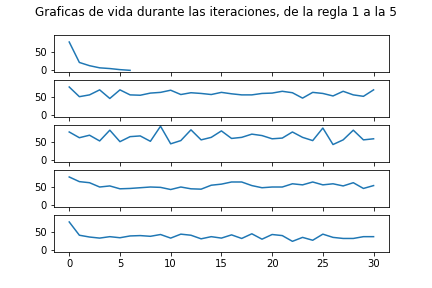
\includegraphics[width=140mm]{Grafica de vida.png}
\caption{\label{fig1}Gráfica de las 5 reglas de supervivencia.}
\end{figure}
\newpage
A continuación, se muestran el estado inicial y final del comportamiento de la matriz para cada regla. Las imagenes en .gif para poder observar bien el proceso en las 30 iteraciones se encuentra en el Github \cite{Denisse_Leyva}.

\begin{figure}[h!]
\centering
\begin{subfigure}[b]{0.45\linewidth}
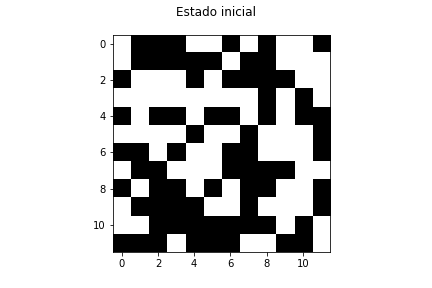
\includegraphics[width=\linewidth]{p2_r1_t00_p.png}
\caption{Estado Inicial}
\end{subfigure}
\begin{subfigure}[b]{0.45\linewidth}
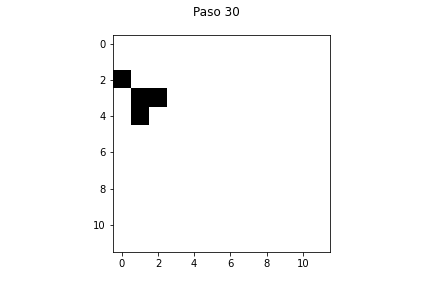
\includegraphics[width=\linewidth]{p2_r1_t30_p.png}
\caption{Estado Final}
\end{subfigure}
\caption{Imagen del estado inicial y final de la regla 1 de supervivencia}
\label{fig:westminster}
\end{figure}


\begin{figure}[H]
\centering
\begin{subfigure}[b]{0.45\linewidth}
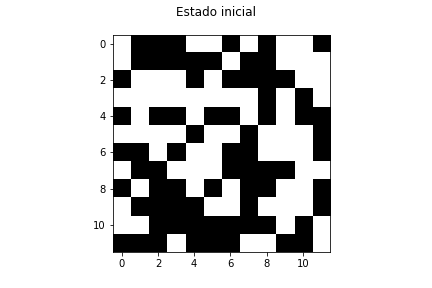
\includegraphics[width=\linewidth]{p2_r2_t00_p.png}
\caption{Estado Inicial}
\end{subfigure}
\begin{subfigure}[b]{0.45\linewidth}
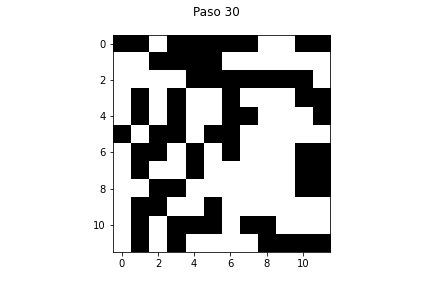
\includegraphics[width=\linewidth]{p2_r2_t30_p.png}
\caption{Estado Final}
\end{subfigure}
\caption{Imagen del estado inicial y final de la regla 2 de supervivencia}
\label{fig:westminster}
\end{figure}

\begin{figure}[H]
\centering
\begin{subfigure}[b]{0.45\linewidth}
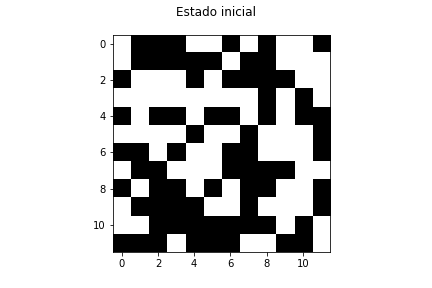
\includegraphics[width=\linewidth]{p2_r3_t00_p.png}
\caption{Estado Inicial}
\end{subfigure}
\begin{subfigure}[b]{0.45\linewidth}
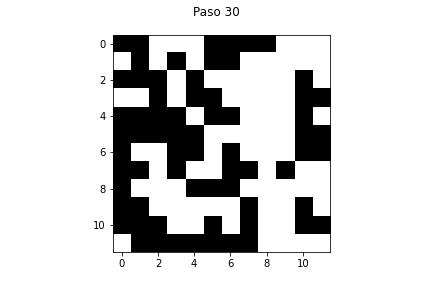
\includegraphics[width=\linewidth]{p2_r3_t30_p.png}
\caption{Estado Final}
\end{subfigure}
\caption{Imagen del estado inicial y final de la regla 3 de supervivencia}
\label{fig:westminster}
\end{figure}

\begin{figure}[H]
\centering
\begin{subfigure}[b]{0.45\linewidth}
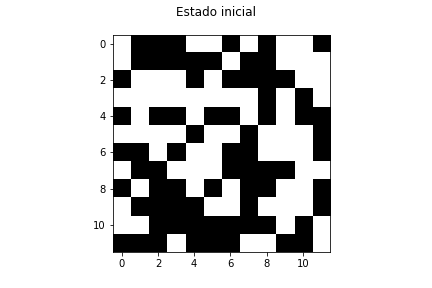
\includegraphics[width=\linewidth]{p2_r4_t00_p.png}
\caption{Estado Inicial}
\end{subfigure}
\begin{subfigure}[b]{0.45\linewidth}
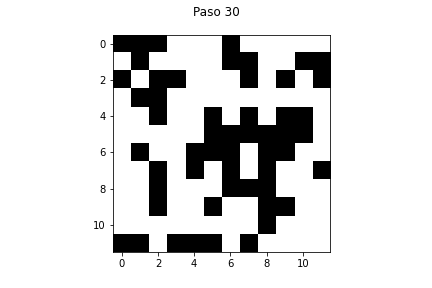
\includegraphics[width=\linewidth]{p2_r4_t30_p.png}
\caption{Estado Final}
\end{subfigure}
\caption{Imagen del estado inicial y final de la regla 4 de supervivencia}
\label{fig:westminster}
\end{figure}

\begin{figure}[H]
\centering
\begin{subfigure}[b]{0.45\linewidth}
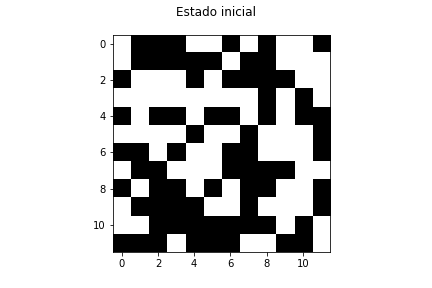
\includegraphics[width=\linewidth]{p2_r5_t00_p.png}
\caption{Estado Inicial}
\end{subfigure}
\begin{subfigure}[b]{0.45\linewidth}
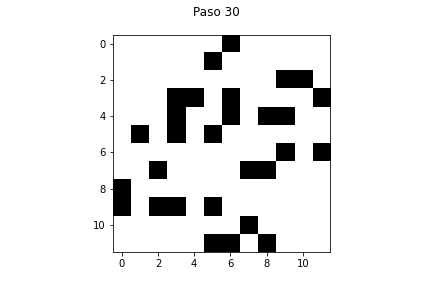
\includegraphics[width=\linewidth]{p2_r5_t30_p.png}
\caption{Estado Final}
\end{subfigure}
\caption{Imagen del estado inicial y final de la regla 5 de supervivencia}
\label{fig:westminster}
\end{figure}


\section{Reto 1}
Para este primer reto se debe modificar la simulación para que modele algún tipo de crecimiento (cristalización) en la microestructura de un material. Los núcleos aparecen al azar en celdas desocupadas y se expanden con una tasa constante a celdas vecinas hasta agotar el espacio disponible. Se debe examinar la distribución de los tamaños de los núcleos que no toquen el borde al finalizar la simulación, eligiendo el tamaño de la zona y el número de semillas de tal forma que sean por lo menos la mitad.

\begin{lstlisting}[language=Python, caption= Código para creación y posicionamiento de semillas.]

dim = 100
semilla = 40
num = dim**2
semill = [x for x in range(1,semilla+1)]
valores = [0 for x in range(num)]
valores[:semilla] = semill
random.shuffle(valores)
actual = np.reshape(valores,(dim,dim))
\end{lstlisting}
\newpage
\begin{lstlisting}[language=Python, caption= Código para expansión de semillas.]

while 0 in m:
    valor = []
    for pos in range(num):
        fila = pos // dim
        columna = pos % dim
        na = actual[fila,columna]
        if na > 0:
            while True:    
                for f in range(max(0, fila -1),min(dim, fila + 2)):
                    for c in range(max(0, columna -1),min(dim, columna +2)):
                       if actual_n[f,c] == 0:
                            actual_n[f,c] = na
                ac = actual_n[max(0, fila -1):min(dim, fila + 2),
                              max(0, columna -1):min(dim, columna +2)].ravel()
                acc = np.count_nonzero(ac == 0)
                if acc == 0:
                    break
    for i in range(num):
        f = i // dim
        c = i % dim
        valor.append(actual_n[f,c])
\end{lstlisting}

\begin{lstlisting}[language=Python, caption= Código para eliminar la orilla]
for i in actual[0,:]:
    no.append(i)
for i in actual[:,0]:
    no.append(i)
for i in actual[dim-1,:]:
    no.append(i)
for i in actual[:,dim-1]:
    no.append(i)
no = np.unique(no)
for i in range(len(no)):
    for x in range(len(valor)):
        a = no[i]
        b = valor[x]
        if a == b:
            valor[x] = 0
\end{lstlisting}

Para mostrar la cristalización que se produjo se creó un archivo tipo gif que se encuentra en el repositorio junto con el código completo\cite{Denisse_Leyva}.

En la figura 8 (a) se muestra la imagen del crecimiento total de las semillas y la 8 (b) eliminando las semillas que tocaron el borde.
Para la figura 8 (b) se elimino el 50.73\% de la zona. 

\begin{figure}[H]
\centering
\begin{subfigure}[b]{0.45\linewidth}
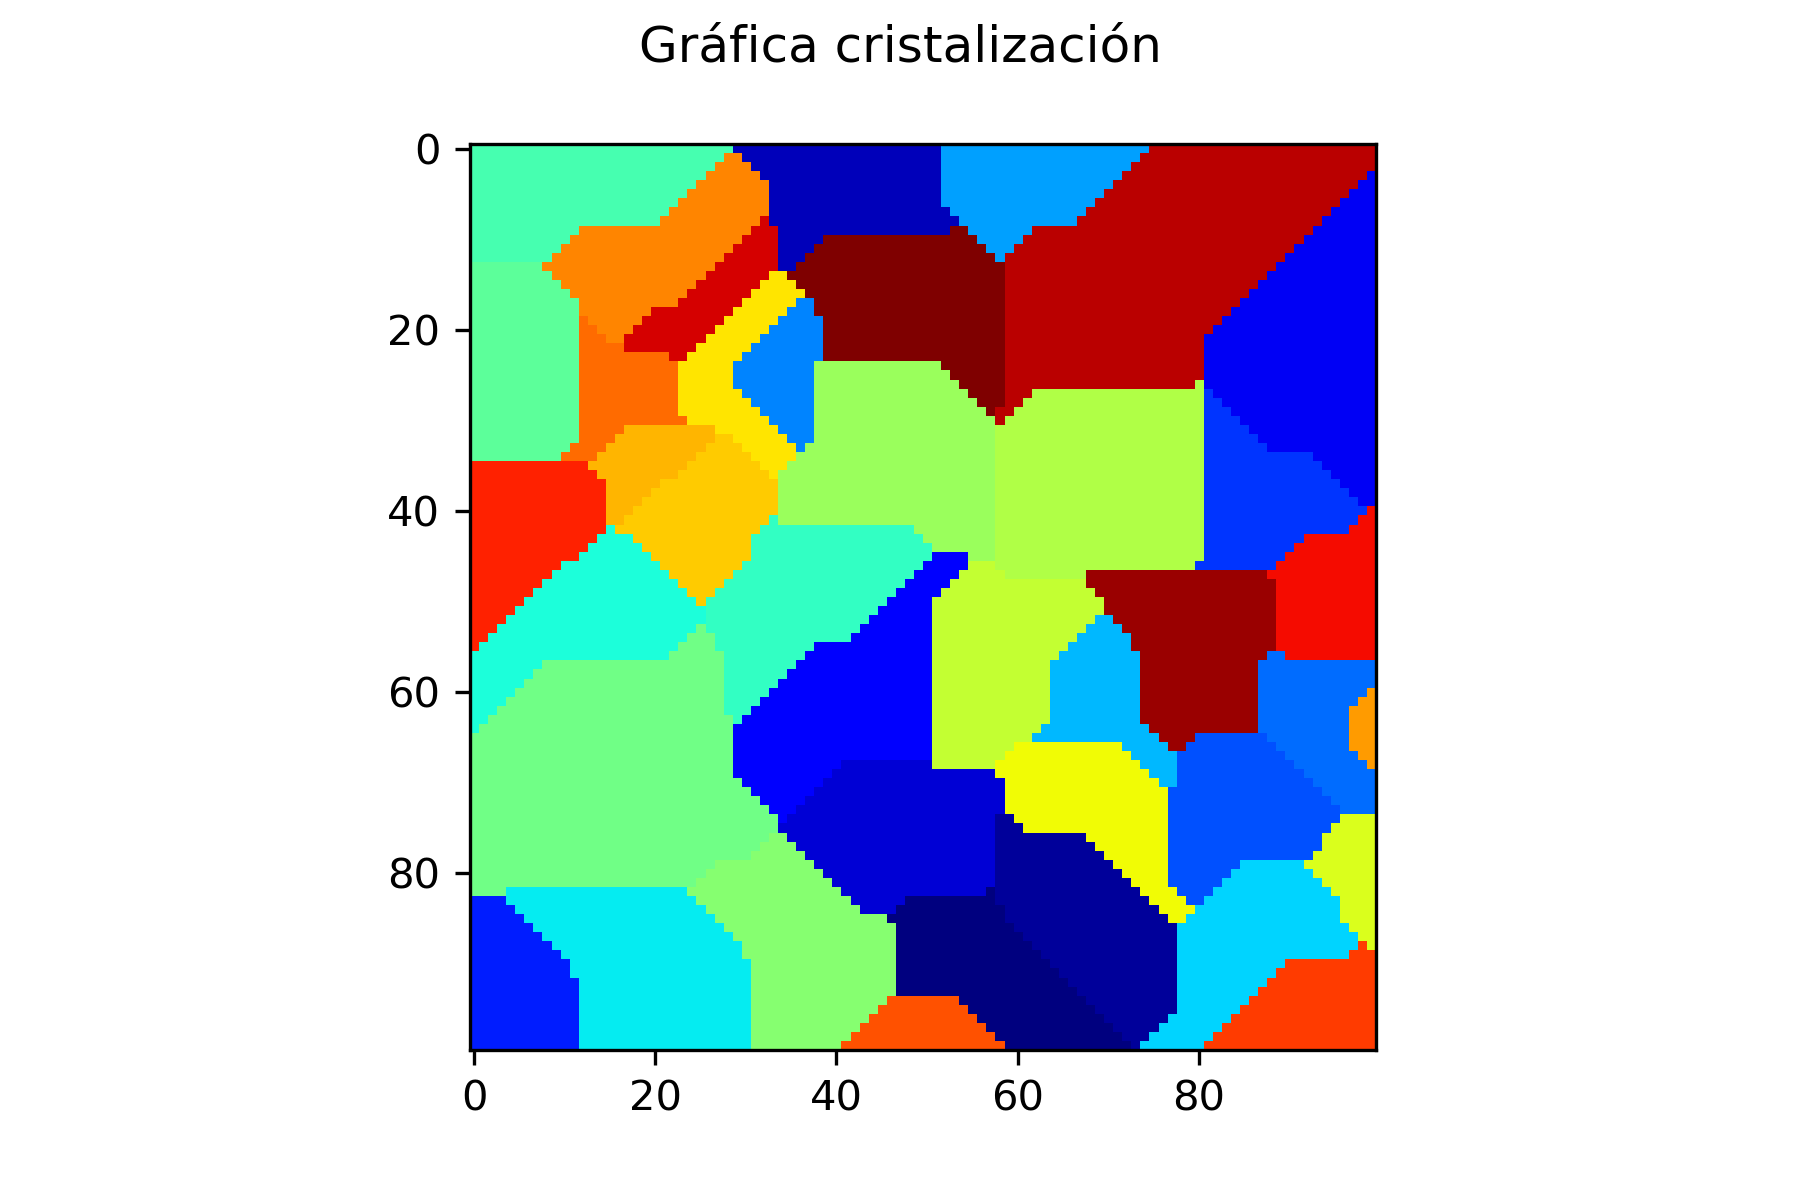
\includegraphics[width=\linewidth]{Reto1_Practica2_29.png}
\caption{Crecimiento total}
\end{subfigure}
\begin{subfigure}[b]{0.45\linewidth}
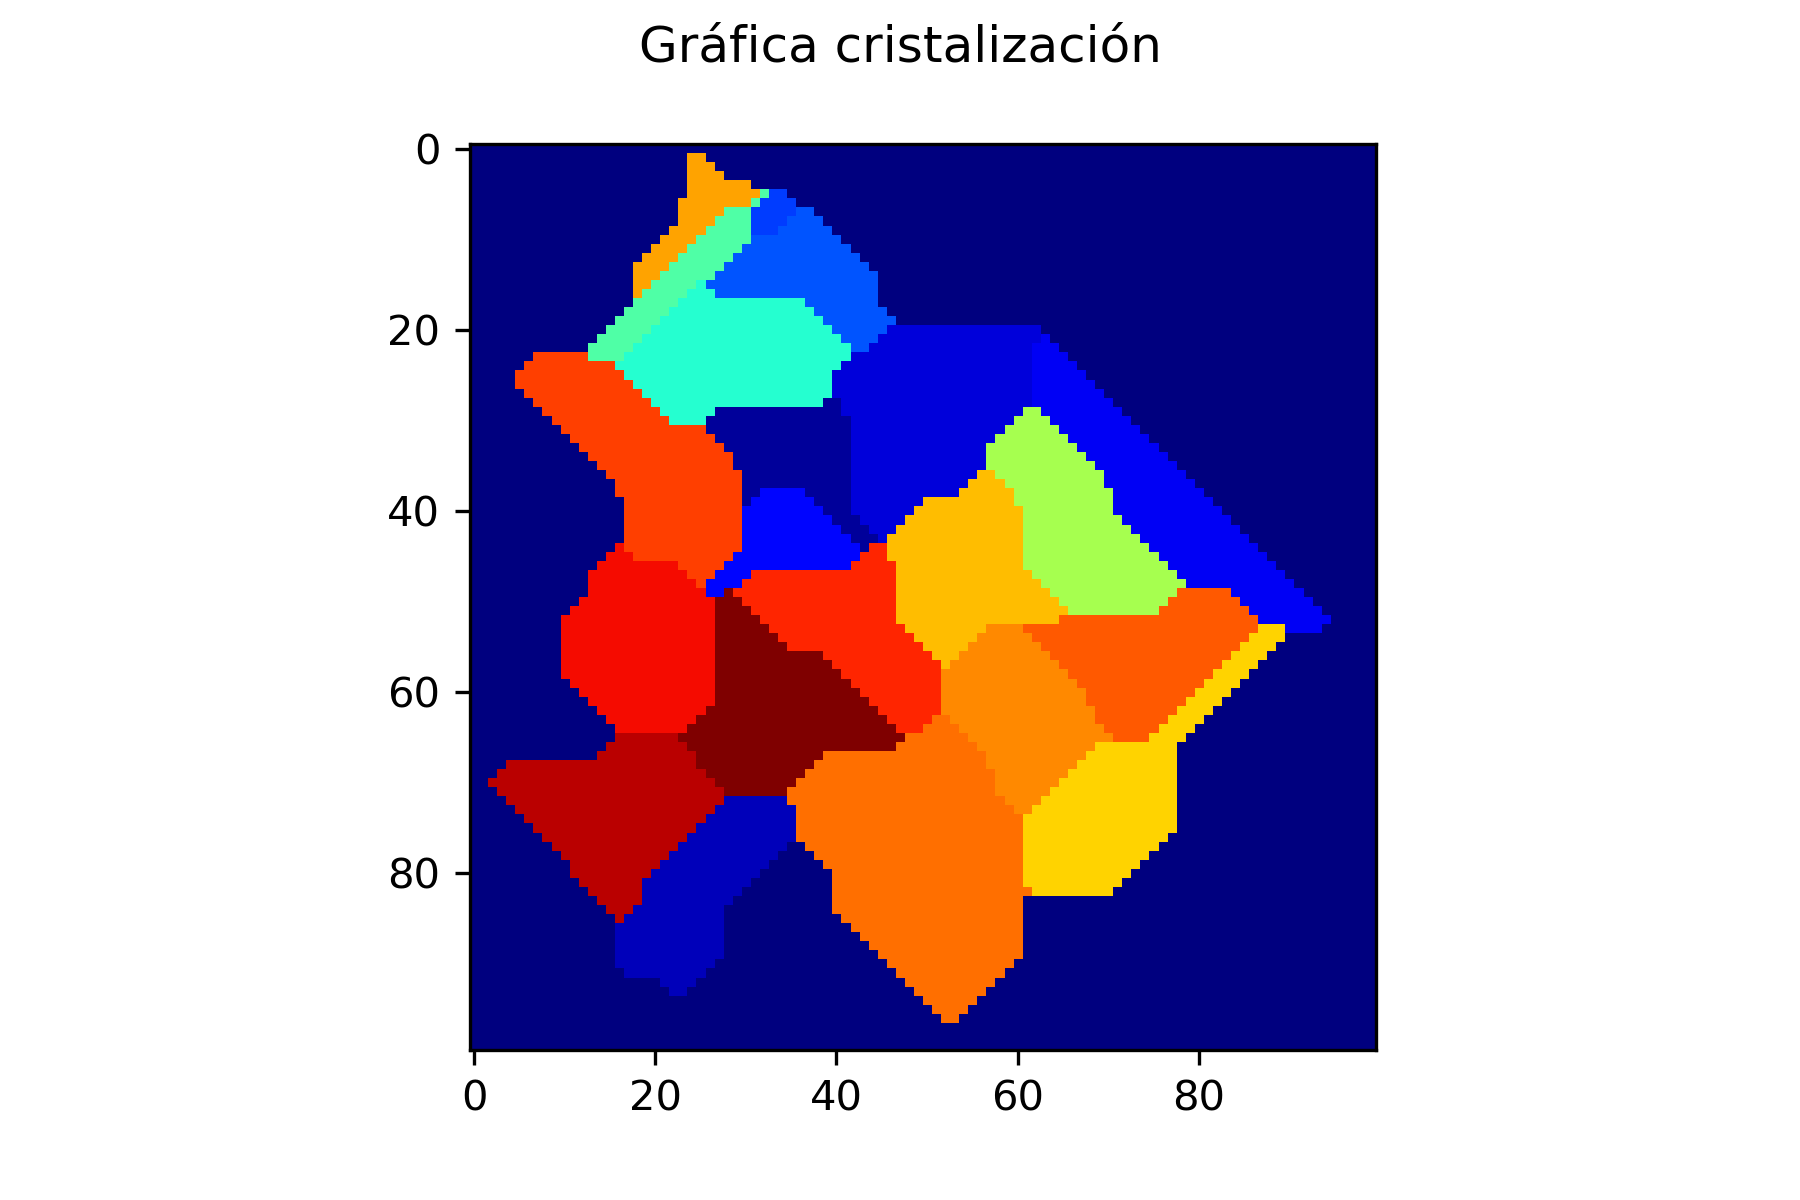
\includegraphics[width=\linewidth]{Reto1_Practica2_f.png}
\caption{Eliminación de las semillas que tocaron el borde}
\end{subfigure}
\caption{Imagen de cristalización}
\label{fig:westminster}
\end{figure}

\section{Reto 2}
Para este segundo reto se ejecutará un autómata celular en un modelo tridimensional.\\
La regla de supervivencia propuesta para este código toma el estado en el que se encuentra la mayoría de sus vecinos es decir si tiene más de dos vecinos en "true" su valor será "true" de no ser así será "false.

En las imágenes de la 9 a la 11 podemos visualizar mejor la regla anterior con el color azul que representa el "true" y el color rojo a "false".
El código completo para la obtención de estas imagenes se encuentra en Github \cite{Denisse_Leyva}.

\begin{figure}[H]
\centering
\begin{subfigure}[b]{0.45\linewidth}
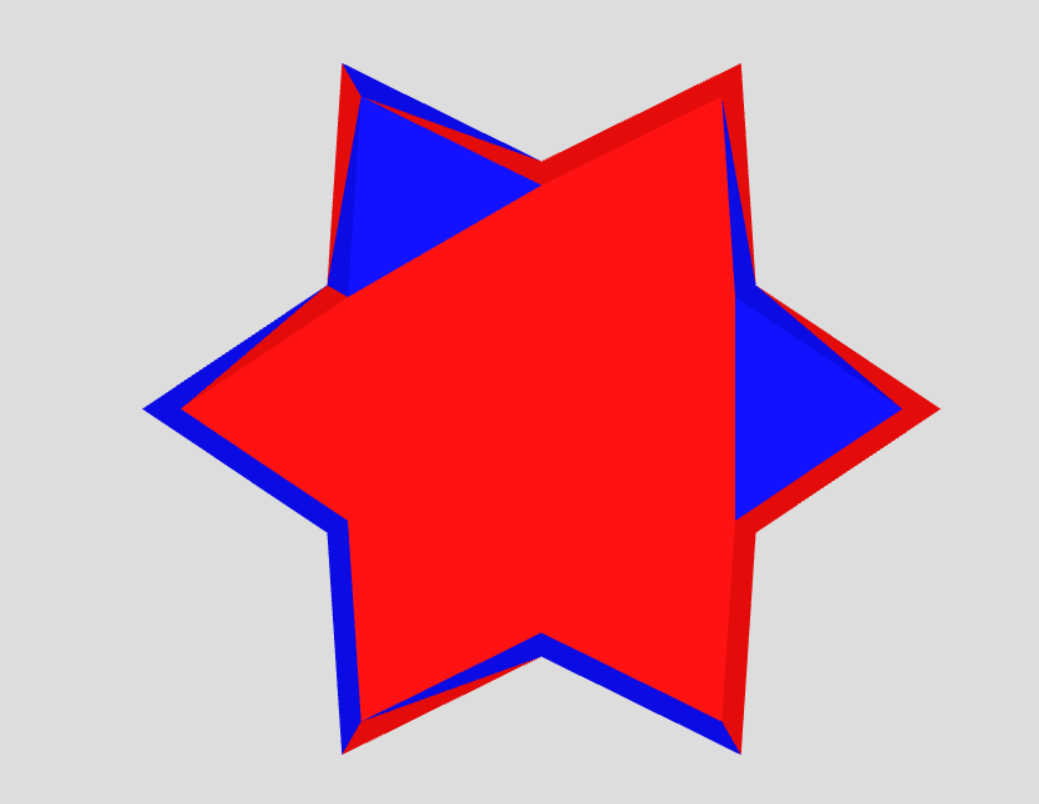
\includegraphics[width=\linewidth]{star_1.png}
\caption{Frontal}
\end{subfigure}
\begin{subfigure}[b]{0.45\linewidth}
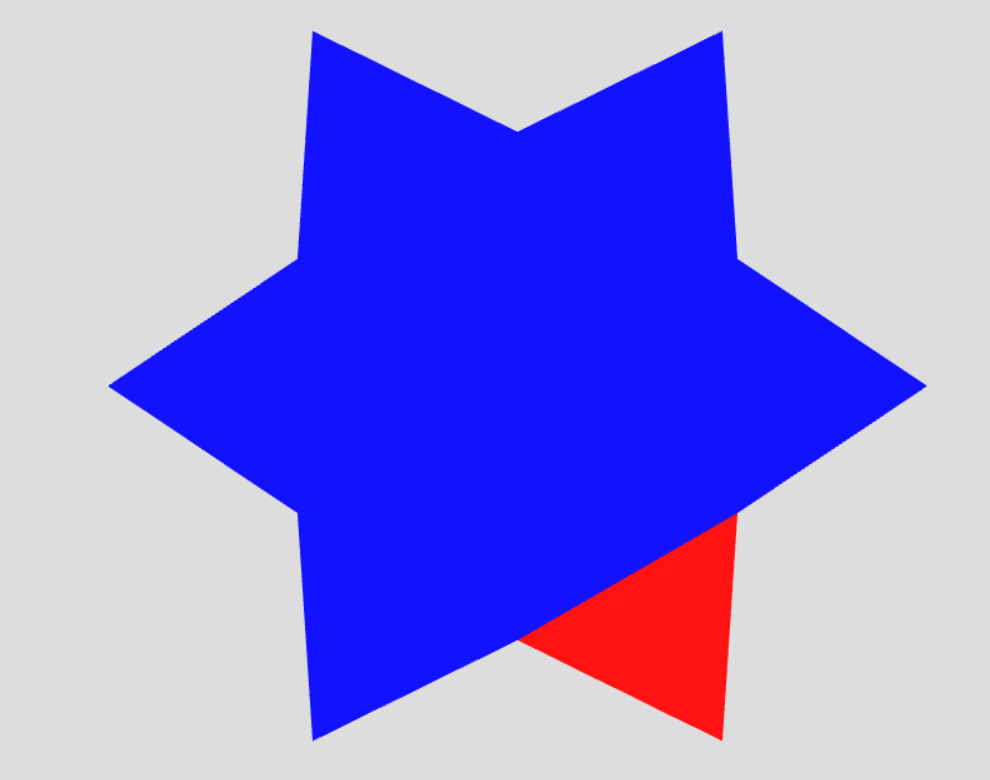
\includegraphics[width=\linewidth]{star_1_1.png}
\caption{Trasera}
\end{subfigure}
\caption{Estado Inicial}
\label{fig:westminster}
\end{figure}

\begin{figure}[H]
\centering
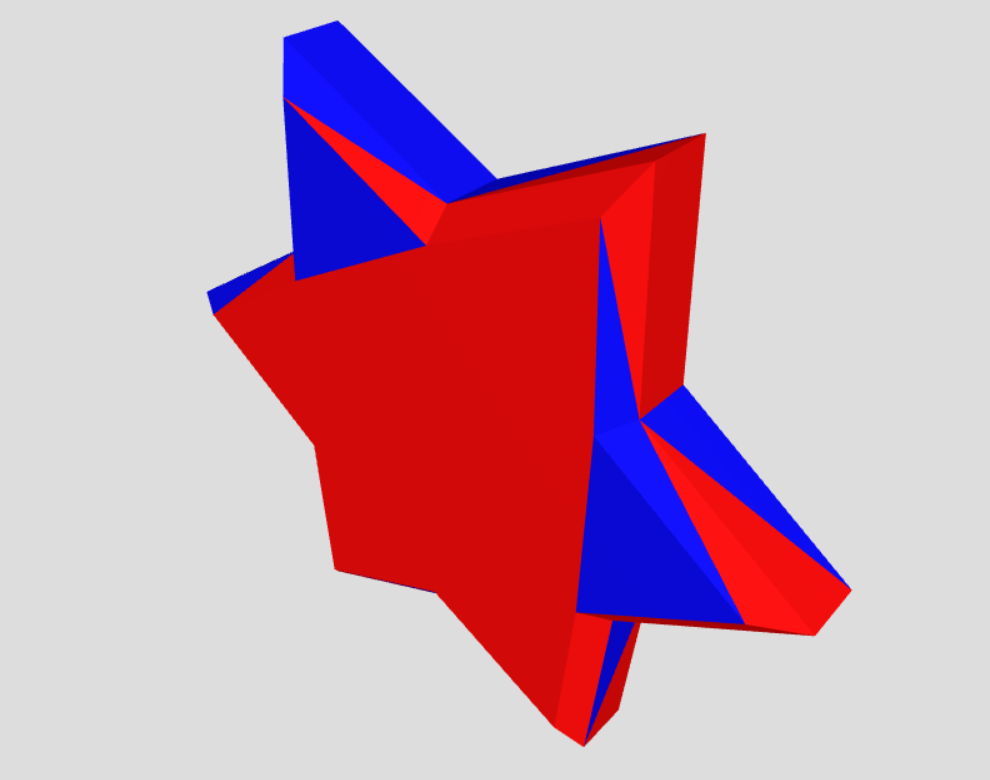
\includegraphics[width=80mm]{star_1_2.png}
\caption{\label{fig1}Isométrica}
\end{figure}

\begin{figure}[H]
\centering
\begin{subfigure}[b]{0.45\linewidth}
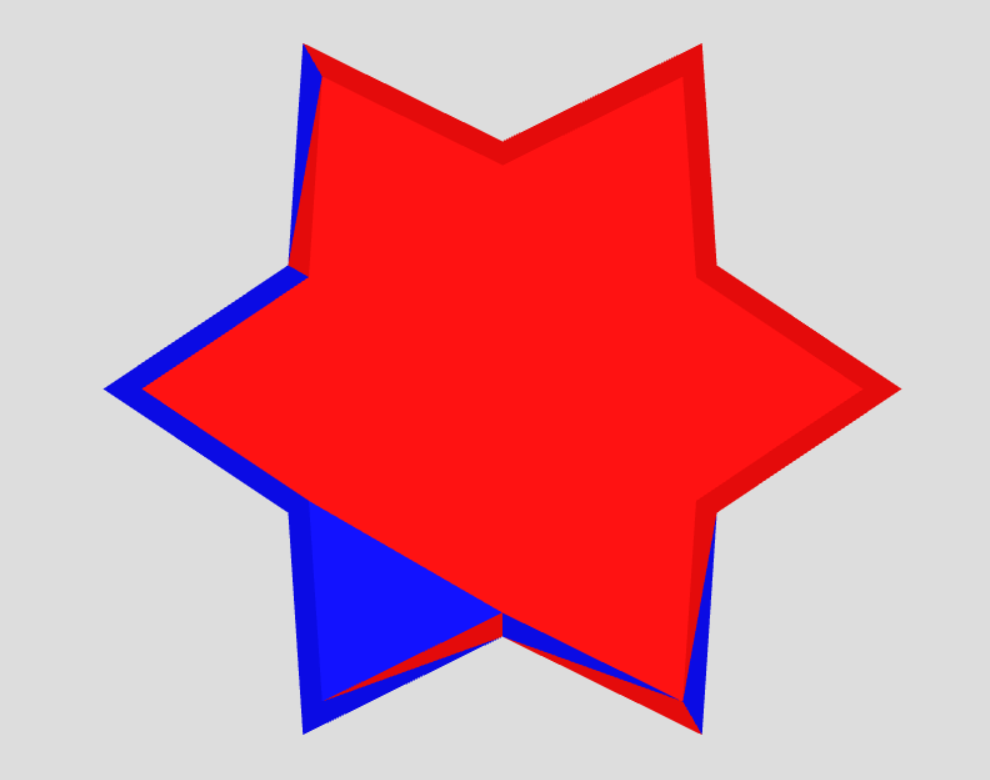
\includegraphics[width=\linewidth]{star_6.png}
\caption{Frontal}
\end{subfigure}
\begin{subfigure}[b]{0.45\linewidth}
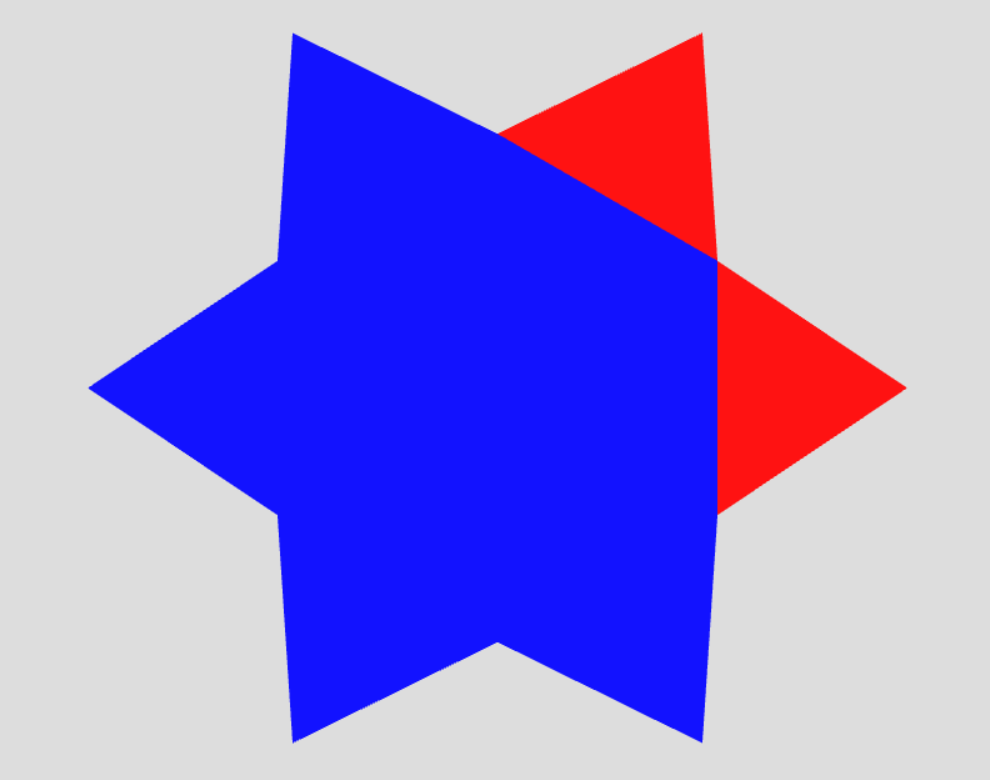
\includegraphics[width=\linewidth]{star_6_1.png}
\caption{Trasera}
\end{subfigure}
\caption{Estado Final}
\label{fig:westminster}
\end{figure}

\begin{figure}[H]
\centering
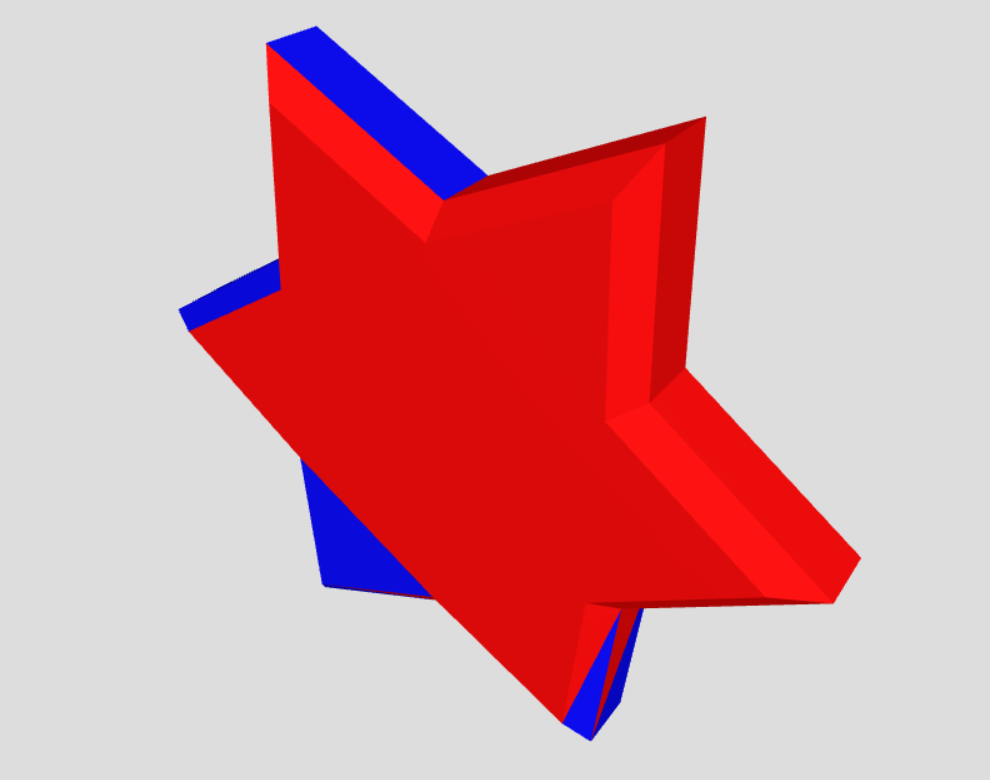
\includegraphics[width=80mm]{star_6_2.png}
\caption{\label{fig1}Isométrica}
\end{figure}

\printbibliography
\end{document}
